\documentclass[a4paper, 12pt]{extreport}

\usepackage[T2A]{fontenc}
\usepackage[utf8]{inputenc}
\usepackage[english,russian]{babel}
\usepackage{amssymb,amsfonts,amsmath,mathtext,cite,enumerate,float}
\usepackage{pgfplots}
\usepackage{graphicx}
\usepackage{tocloft}
\usepackage{listings}
\usepackage{caption}
\usepackage{tempora}
\usepackage{titlesec}
\usepackage{setspace}
\usepackage{geometry}
\usepackage{indentfirst}
\usepackage{pdfpages}
\usepackage{enumerate,letltxmacro}
\usepackage{threeparttable}
\usepackage{hyperref}
\usepackage{flafter}
\usepackage{enumitem}
\usepackage{multirow}
\usepackage{float}
%\usepackage[newfloat]{minted}
\usepackage[figure,table]{totalcount}
\usepackage{lastpage}

\setlist{nosep}

\newcommand{\ssr}[1]{\begin{center}
		\LARGE\bfseries{#1}
	\end{center} \addcontentsline{toc}{chapter}{#1}  }

\makeatletter
\renewcommand\LARGE{\@setfontsize\LARGE{22pt}{20}}
\renewcommand\Large{\@setfontsize\Large{20pt}{20}}
\renewcommand\large{\@setfontsize\large{16pt}{20}}
\makeatother
\RequirePackage{titlesec}
\titleformat{\chapter}[block]{\hspace{\parindent}\large\bfseries}{\thechapter}{0.5em}{\large\bfseries\raggedright}
\titleformat{name=\chapter,numberless}[block]{\hspace{\parindent}}{}{0pt}{\large\bfseries\centering}
\titleformat{\section}[block]{\hspace{\parindent}\large\bfseries}{\thesection}{0.5em}{\large\bfseries\raggedright}
\titleformat{\subsection}[block]{\hspace{\parindent}\large\bfseries}{\thesubsection}{0.5em}{\large\bfseries\raggedright}
\titleformat{\subsubsection}[block]{\hspace{\parindent}\large\bfseries}{\thesubsection}{0.5em}{\large\bfseries\raggedright}
\titlespacing{\chapter}{12.5mm}{-22pt}{10pt}
\titlespacing{\section}{12.5mm}{10pt}{10pt}
\titlespacing{\subsection}{12.5mm}{10pt}{10pt}
\titlespacing{\subsubsection}{12.5mm}{10pt}{10pt}

\makeatletter
\renewcommand{\@biblabel}[1]{#1.}
\makeatother
%
%\titleformat{\chapter}[hang]{\LARGE\bfseries}{\hspace{1.25cm}\thechapter}{1ex}{\LARGE\bfseries}
%\titleformat{\section}[hang]{\Large\bfseries}{\hspace{1.25cm}\thesection}{1ex}{\Large\bfseries}
%\titleformat{name=\section,numberless}[hang]{\Large\bfseries}{\hspace{1.25cm}}{0pt}{\Large\bfseries}
%\titleformat{\subsection}[hang]{\large\bfseries}{\hspace{1.25cm}\thesubsection}{1ex}{\large\bfseries}
%\titlespacing{\chapter}{0pt}{-\baselineskip}{\baselineskip}
%\titlespacing*{\section}{0pt}{\baselineskip}{\baselineskip}
%\titlespacing*{\subsection}{0pt}{\baselineskip}{\baselineskip}
 
\geometry{left=30mm}
\geometry{right=10mm}
\geometry{top=20mm}
\geometry{bottom=20mm}

\onehalfspacing

\renewcommand{\theenumi}{\arabic{enumi}}
\renewcommand{\labelenumi}{\arabic{enumi}\text{)}}
\renewcommand{\theenumii}{.\arabic{enumii}}
\renewcommand{\labelenumii}{\asbuk{enumii}\text{)}}
\renewcommand{\theenumiii}{.\arabic{enumiii}}
\renewcommand{\labelenumiii}{\arabic{enumi}.\arabic{enumii}.\arabic{enumiii}.}
\renewcommand{\cftchapleader}{\cftdotfill{\cftdotsep}}

\addto\captionsrussian{\renewcommand{\figurename}{Рисунок}}
\DeclareCaptionLabelSeparator{dash}{~---~}
\captionsetup{labelsep=dash}

\captionsetup[figure]{justification=centering,labelsep=dash}
\captionsetup[table]{labelsep=dash,justification=raggedright,singlelinecheck=off}

\graphicspath{{images/}}%путь к рисункам

\newcommand{\floor}[1]{\lfloor #1 \rfloor}

\lstset{ %
	language={[x86masm]Assembler},                 % выбор языка для подсветки (здесь это С)
	basicstyle=\scriptsize, % размер и начертание шрифта для подсветки кода
	numbers=left,               % где поставить нумерацию строк (слева\справа
	numberstyle=\scriptsize,           % размер шрифта для номеров строк
	stepnumber=1,                   % размер шага между двумя номерами строк
	numbersep=5pt,                % как далеко отстоят номера строк от подсвечиваемого кода
	showspaces=false,            % показывать или нет пробелы специальными отступами
	showstringspaces=false,      % показывать или нет пробелы в строках
	showtabs=true,             % показывать или нет табуляцию в строках
	tab=\quad,
	frame=single,              % рисовать рамку вокруг кода
	tabsize=2,                 % размер табуляции по умолчанию равен 2 пробелам
	captionpos=t,              % позиция заголовка вверху [t] или внизу [b] 
	breaklines=true,           % автоматически переносить строки (да\нет)
	breakatwhitespace=false, % переносить строки только если есть пробел
	escapeinside={\#*}{*)},   % если нужно добавить комментарии в коде
	abovecaptionskip=-5pt,
	captionpos=b
}



\pgfplotsset{width=0.85\linewidth, height=0.5\columnwidth}

\linespread{1.3}

\parindent=1.25cm

%\LetLtxMacro\itemold\item
%\renewcommand{\item}{\itemindent0.75cm\itemold}

\def\labelitemi{---}
\setlist[itemize]{leftmargin=1.25cm, itemindent=0.65cm}
\setlist[enumerate]{leftmargin=1.25cm, itemindent=0.55cm}

\newcommand{\specialcell}[2][c]{%
	\begin{tabular}[#1]{@{}c@{}}#2\end{tabular}}

\frenchspacing
\begin{document}
	\thispagestyle{empty}
	
	\noindent \begin{minipage}{0.15\textwidth}
		
\includegraphics[width=\linewidth]{b_logo}
	\end{minipage}
	\noindent\begin{minipage}{0.85\textwidth}\centering
		\textbf{Министерство науки и высшего образования Российской Федерации}\\
		\textbf{Федеральное государственное бюджетное образовательное учреждение высшего образования}\\
		\textbf{«Московский государственный технический университет имени Н.Э.~Баумана}\\
		\textbf{(национальный исследовательский университет)»}\\
		\textbf{(МГТУ им. Н.Э.~Баумана)}
	\end{minipage}
	
	\noindent\rule{\linewidth}{3pt}
	\newline\newline
	\noindent ФАКУЛЬТЕТ $\underline{\text{«ИНФОРМАТИКА И СИСТЕМЫ УПРАВЛЕНИЯ»}}$ \newline\newline
	\noindent КАФЕДРА $\underline{\text{«ПРОГРАММНОЕ ОБЕСПЕЧЕНИЕ ЭВМ И ИНФОРМАЦИОННЫЕ ТЕХНОЛОГИИ»}}$
	
	\vspace{1cm}
	
	\begin{center}
		\noindent\begin{minipage}{1.3\textwidth}\centering
			\Large\textbf{  Лабораторная работа № 1}\newline
			\textbf{по дисциплине <<Операционные системы>>}\newline\newline
		\end{minipage}
	\end{center}
	
	\noindent\textbf{Тема} $\underline{\text{Прерывание INT 8h}}$\newline\newline
	\noindent\textbf{Студент} $\underline{\text{Бугаков И. С.}}$\newline\newline
	\noindent\textbf{Группа} $\underline{\text{ИУ7-54Б}}$\newline\newline
	\noindent\textbf{Преподаватель} $\underline{\text{Рязанова Н. Ю.}}$\newline
	
	\begin{center}
		\vfill
		Москва,~\the\year
	\end{center}
	\clearpage
	
	\chapter{Дизассемблированный код}
		\section{Обработчик прерывания INT 8h}
		{\linespread{1.2}
		\begin{lstlisting}[caption={Обработчик прерывания INT 8h}]
			020C:0746  E8 0070          call	sub_1                   ; (07B9)
			020C:0749  06               push	es
			020C:074A  1E               push	ds
			020C:074B  50               push	ax
			020C:074C  52               push	dx
			020C:074D  B8 0040          mov		ax,40h
			020C:0750  8E D8            mov		ds,ax
			020C:0752  33 C0            xor		ax,ax                   ; Zero register
			020C:0754  8E C0            mov		es,ax
			020C:0756  FF 06 006C       inc		word ptr ds:[6Ch]       ; (0040:006C=1808h)
			020C:075A  75 04            jnz		loc_1                   ; Jump if not zero
			020C:075C  FF 06 006E       inc		word ptr ds:[6Eh]       ; (0040:006E=0Dh)
			020C:0760			loc_1:                                      ;  xref 020C:075A
			020C:0760  83 3E 006E 18    cmp		word ptr ds:[6Eh],18h   ; (0040:006E=0Dh)
			020C:0765  75 15            jne		loc_2                   ; Jump if not equal
			020C:0767  81 3E 006C 00B0  cmp		word ptr ds:[6Ch],0B0h  ; (0040:006C=1808h)
			020C:076D  75 0D            jne		loc_2                   ; Jump if not equal
			020C:076F  A3 006E          mov		word ptr ds:[6Eh],ax    ; (0040:006E=0Dh)
			020C:0772  A3 006C          mov		word ptr ds:[6Ch],ax    ; (0040:006C=1808h)
			020C:0775  C6 06 0070 01    mov		byte ptr ds:[70h],1     ; (0040:0070=0)
			020C:077A  0C 08            or		al,8
			020C:077C			loc_2:                                      ;  xref 020C:0765, 076D
			020C:077C  50               push	ax
			020C:077D  FE 0E 0040       dec		byte ptr ds:[40h]       ; (0040:0040=7Dh)
			020C:0781  75 0B            jnz		loc_3                   ; Jump if not zero
			020C:0783  80 26 003F F0    and		byte ptr ds:[3Fh],0F0h  ; (0040:003F=0)
			020C:0788  B0 0C            mov		al,0Ch
			020C:078A  BA 03F2          mov		dx,3F2h
			020C:078D  EE               out		dx,al                   ; port 3F2h, dsk0 contrl output
			020C:078E			loc_3:                                      ; xref 020C:0781
			020C:078E  58               pop		ax
			020C:078F  F7 06 0314 0004  test	word ptr ds:[314h],4    ; (0040:0314=3200h)
			020C:0795  75 0C            jnz		loc_4                   ; Jump if not zero
			020C:0797  9F               lahf                            ; Load ah from flags
			020C:0798  86 E0            xchg	ah,al
			020C:079A  50               push	ax
			020C:079B  26: FF 1E 0070   call	dword ptr es:[70h]      ; (0000:0070=6ADh)
			020C:07A0  EB 03            jmp		short loc_5             ; (07A5)
			020C:07A2  90               nop
			020C:07A3			loc_4:                                      ;  xref 020C:0795
			020C:07A3  CD 1C            int		1Ch                     ; Timer break (call each 18.2ms)
			020C:07A5			loc_5:                                      ;  xref 020C:07A0
			020C:07A5  E8 0011          call	sub_1                   ; (07B9)
			020C:07A8  B0 20            mov		al,20h                  ; ' '
			020C:07AA  E6 20            out		20h,al                  ; port 20h, 8259-1 int command                                                             ; al = 20h, end of interrupt
			020C:07AC  5A               pop		dx
			020C:07AD  58               pop		ax
			020C:07AE  1F               pop		ds
			020C:07AF  07               pop		es
			020C:07B0  E9 FE99          jmp		$-164h
			; <...>
			020C:0D93  CF               iret                            ; Interrupt return		\end{lstlisting}}
		\section{Процедура sub\_1}
		{\linespread{1.2}
		\noindent\begin{lstlisting}[caption={Процедура sub\_1}]
							sub_1		    proc        near
			020C:07B9  1E                   push        ds
			020C:07BA  50                   push        ax
			020C:07BB  B8 0040              mov         ax,40h
			020C:07BE  8E D8                mov         ds,ax
			020C:07C0  9F                   lahf                                    ; Load ah from flags
			020C:07C1  F7 06 0314 2400      test        word ptr ds:[314h],2400h	  ; (0040:0314=3200h)
			020C:07C7  75 0C                jnz	        loc_7			                  ; Jump if not zero
			020C:07C9  F0> 81 26 0314 FDFF  lock and	word ptr ds:[314h],0FDFFh	    ; (0040:0314=3200h)
			020C:07D0			loc_6:						                                        ;  xref 020C:07D6
			020C:07D0  9E                   sahf                                    ; Store ah into flags
			020C:07D1  58                   pop         ax
			020C:07D2  1F                   pop         ds
			020C:07D3  EB 03                jmp short   loc_ret_8		                ; (07D8)
			020C:07D5			loc_7:                                                    ;  xref 020C:07C7
			020C:07D5  FA                   cli                                     ; Disable interrupts
			020C:07D6  EB F8                jmp short   loc_6                       ; (07D0)
			
			020C:07D8			loc_ret_8:                                                ;  xref 020C:07D3
			020C:07D8  C3                   retn
			        sub_1       endp		
		\end{lstlisting}}
	\chapter{Схемы алгоритмов}
	\section{Схема алгоритма обработчика прерывания INT 8h}
	\begin{figure}[H]
		\centering
		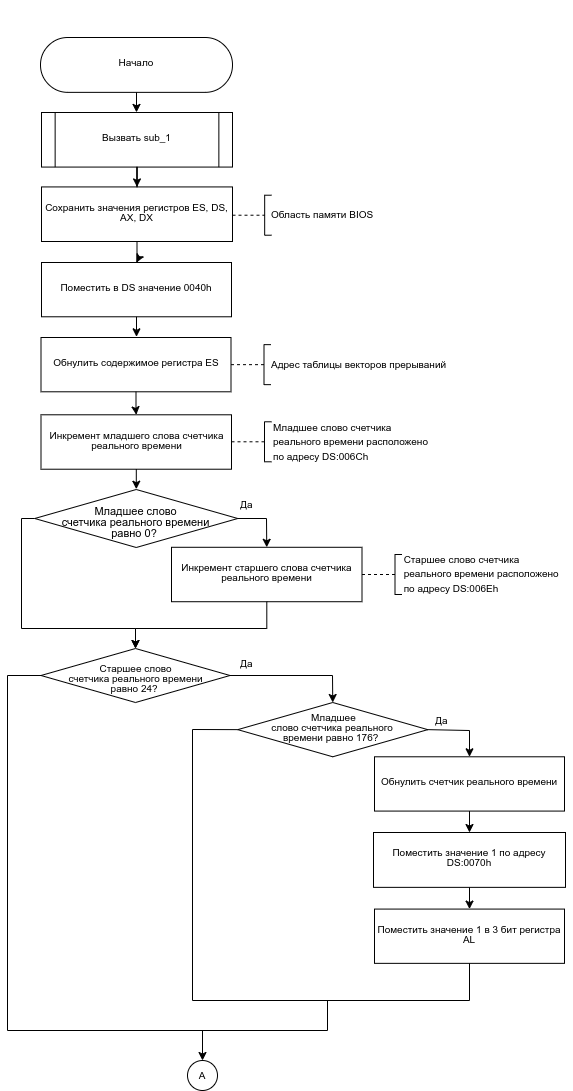
\includegraphics[width=0.7\linewidth]{Int_8h_part1.png}
	\end{figure}
	\begin{figure}[H]
		\centering
		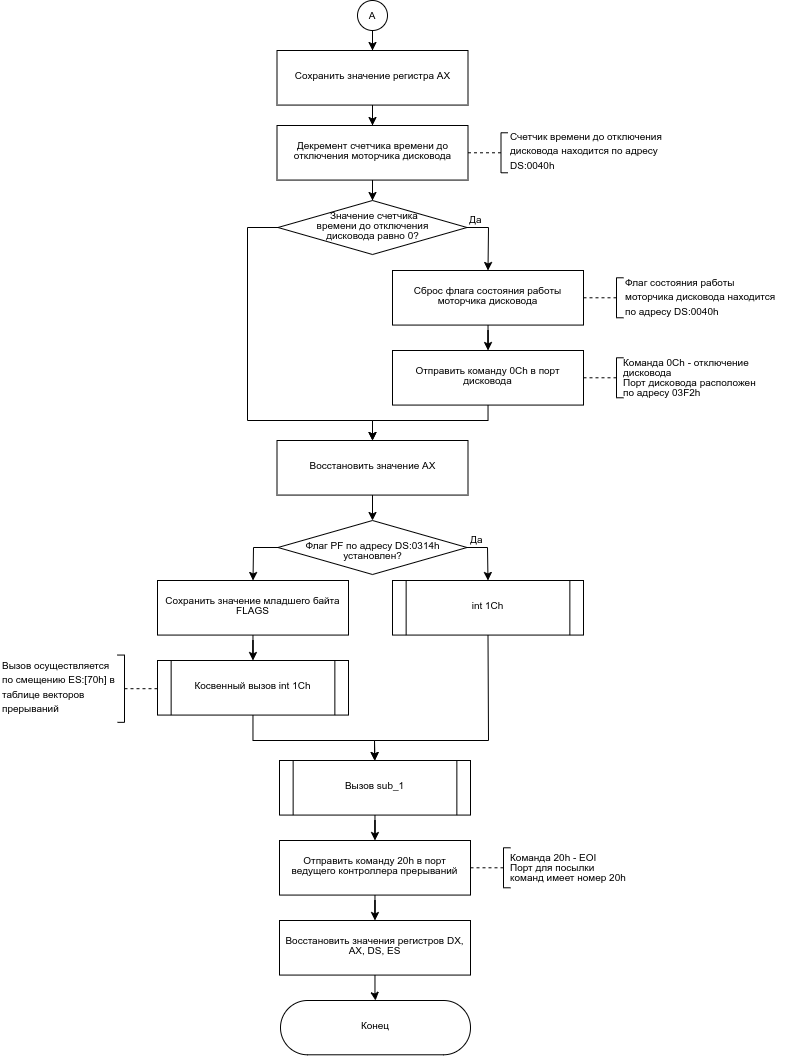
\includegraphics[width=\linewidth]{Int_8h_part2.png}
	\end{figure}
	\section{Схема алгоритма подпрограммы sub\_1}
	\begin{figure}[H]
		\centering
		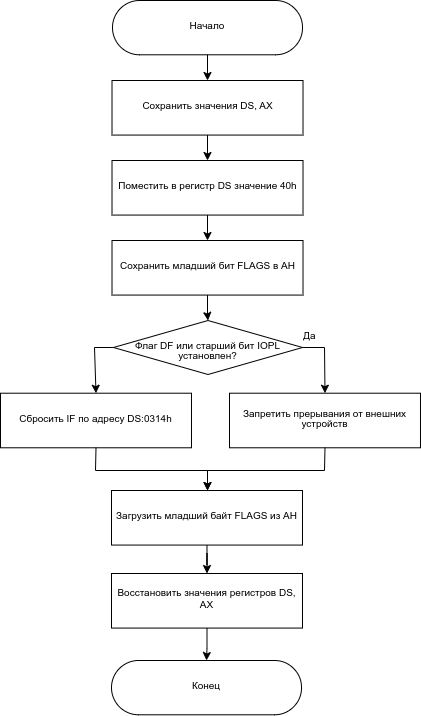
\includegraphics[width=0.7\linewidth]{subroutine.png}
	\end{figure}
\end{document}